%==============================================================================
% Sjabloon onderzoeksvoorstel bachelorproef
%==============================================================================%
% Compileren in TeXstudio:
%
% - Zorg dat Biber de bibliografie compileert (en niet Biblatex)
%   Options > Configure > Build > Default Bibliography Tool: "txs:///biber"
% - F5 om te compileren en het resultaat te bekijken.
% - Als de bibliografie niet zichtbaar is, probeer dan F5 - F8 - F5
%   Met F8 compileer je de bibliografie apart.
%
% Als je JabRef gebruikt voor het bijhouden van de bibliografie, zorg dan
% dat je in ``biblatex''-modus opslaat: File > Switch to BibLaTeX mode.

\documentclass{hogent-article}
\usepackage{graphicx}
\usepackage{lipsum} % Voor vultekst


%------------------------------------------------------------------------------
% Metadata over het artikel
%------------------------------------------------------------------------------

%---------- Titel & auteur ----------------------------------------------------

% TODO: (fase 2) geef werktitel van je eigen voorstel op
\PaperTitle{machine learning applicatie voor de detectie  van slaap bruxisme}
% Dit is typisch de opdracht en het vak waarvoor dit artikel geschreven is, bv.
% ``Verslag onderzoeksproject Onderzoekstechnieken 2018-2019''
\PaperType{Paper Research Methods: onderzoeksvoorstel}

% TODO: (fase 1) vul je eigen naam in als auteur, geef ook je emailadres mee!
\Authors{Brent De Corte\textsuperscript{1}} % Authors

% Als het hier effectief gaat om een voorstel voor de bachelorproef, dan ben je
% hier verplicht de naam van je co-promotor in te vullen. Zoniet, dan kan je het
% leeg laten.
\CoPromotor{}

% Contactinfo: Geef hier de contactgegevens van elke auteur van het artikel (en
% indien van toepassing ook van de co-promotor).
\affiliation{
  \textsuperscript{1} \href{mailto:brent.decorte@student.hogent.be}{brent.decorte@student.hogent.be}}


%---------- Abstract ----------------------------------------------------------

\Abstract{% TODO: (fase 6)
Dit onderzoek zal zoch focussen op de creatie van een audio detectie deep learning model dat geintegreerd zal worden in een mobiele applicatie die Bruxisme kan herkennen op het feit van het knarsen van tanden .
Het model komt tot stand door de transformatie van audio fragmenten in spectrogrammen met extra tijd en frequency masking zodat het scenario in een image classificatie  probleem verandet kan worden .
Wanneer het model getrained is, zal het worden geimplementeerd in een mobiele applicatie gebaseerd op het python framework Kivy .
}

%---------- Onderzoeksdomein en sleutelwoorden --------------------------------
% TODO: (fase 2) Vul de sleutelwoorden aan.

% Het eerste sleutelwoord beschrijft het onderzoeksdomein. Je kan kiezen uit
% deze lijst:
%
% - Mobiele applicatieontwikkeling
% - Webapplicatieontwikkeling
% - Applicatieontwikkeling (andere)
% - Systeembeheer
% - Netwerkbeheer
% - Mainframe
% - E-business
% - Databanken en big data
% - Machineleertechnieken en kunstmatige intelligentie
% - Andere (specifieer)
%
% De andere sleutelwoorden zijn vrij te kiezen.

\Keywords{Machineleertechnieken en kunstmatige intelligentie; geluid detectie; Bruxisme}
\newcommand{\keywordname}{Sleutelwoorden} % Defines the keywords heading name

%---------- Titel, inhoud -----------------------------------------------------

\bibliography{bibliografie}

\begin{document}



\flushbottom % Makes all text pages the same height
\maketitle % Print the title and abstract box
\tableofcontents % Print the contents section
\thispagestyle{empty} % Removes page numbering from the first page

%------------------------------------------------------------------------------
% Hoofdtekst
%------------------------------------------------------------------------------

\section{Inleiding}

% TODO: (fase 2) introduceer je gekozen onderwerp, formuleer de onderzoeksvraag en deelvragen. Wat is de doelstelling (is die S.M.A.R.T.?), wat zal het resultaat zijn van het onderzoek (een Proof-of-Concept, een prototype, een advies, ...)? Waarom is het nuttig om dit onderwerp te onderzoeken?
Slaap Bruxisme (SB) is het onvrijwillig knarsen en het klemmen van tanden tijden het slapen .
SB kan leiden to een tal van problemen zoals hypertensie, dentuur problemen waaronder het verlies van tandoppervlakte en gebarsten tanden, klachten van partners .
Deze problemen kunnen leiden tot een noemenswaardige daling van de levenskwaliteit, daarom is het essentieel om snel en makkelijk te ontdekken of iemand SB heeft .
\bigbreak
Er zijn op dit moment apparaten om thuis SB to ontdekken op basis van kaak spier metingen of zenuwmetingen, één voorbeeld hiervan is bitestrip \cite{Shochat_2007} .
Deze methode van detectie is adequaat, maar er zijn zekere tekortkomingen, de kost van de apparatuur en de limitaties van de slaap hinder tijdens het detectie proces .
Omdat er tot heden geen eenvoudige manier is om te detecteren of iemand van SB leidt die goedkoop, betrouwbaar en die niet interfereert met met het slaap proces .
\bigbreak
In kort, er is waarde in de creatie van een systeem dat machine learning gebruikt om SB te detecteren die toegankelijk is en makkelijk te gebruiken .






\section{Overzicht literatuur}

% TODO: (fase 4) schrijf de literatuurstudie uit en gebruik waar gepast referenties naar de vakliteratuur.

% Refereren naar de literatuur kan met:
% \autocite{BIBTEXKEY} -> (Auteur, jaartal)
% \textcite{BIBTEXKEY} -> Auteur (jaartal)
%Voorbeeld van een referentie waar de auteursnaam geen onderdeel van de zin is~\autocite{Moore2002}.
Vandaag bestaan er verschillende methodes om SB te ontdekken zoals deze op basis van electromyografie, waarbij elektrische signalen van de zenuwen worden omgezet in interpreteerbare data en het registreren van de hartslag die toeneemt voor een SB aanval \cite{Deregibus_2013}
Ook bestaat er een methode die zich baseert op het meten van kaak spier bewegingen .

Beide van deze methodes zijn gelimiteerd in hun manier van detectie, omdat de patient zijn slaapcomfort vermindert .

Om de opgenomen hoeveelheid data te augmenteren zijn er verschillende methodes 

\begin{itemize}
	\item de drie eerste methodes die omschreven zijn komen uit \cite{Wei_2020}
	
	\item Time streching
	\bigbreak 
	\begin{itemize}
		\item Het verhogen of verlagen van de snelheid waarmee het audiofragment wordt afgespeeld .
		Om de originele inputgrootte van het model te behouden kan zero-padding worden gebruikt als het fragment versneld word of cropping als het fragment vertraagd word .
		 
	\end{itemize}
	\bigbreak
	\item toevoegen van "noise"
	\bigbreak
	\begin{itemize}
		\item De toevoeging van Gauss-ruis met de hyperparameter die the amplitude regelt laat de mogelijkheid om overfitting tegen te gaan . Het gebruik van Gauss-ruis is niet gelimiteerd tot de input maar ook toegevoegd worden aan de andere componenten zoals de activatie functie .
	\end{itemize}
	\bigbreak
	\item pitch shift
	\bigbreak 
	\begin{itemize}
		\item Het verhogen of verlagen van de halve toonafstanden, de kleinste stap omhoog of omlaag van een bestaande toon,  van het audiofragment, hetzelfde concept als het hierboven vermelde Time Stretching  .
			
	\end{itemize}
	\bigbreak

	\item SpecAugment
	\bigbreak
	\begin{itemize}
		\item SpecAugment gebruikt 2 methodes om spectrogrammen to augmenteren .
		het verbergen van een bepaald bereik op de frequenctie schaal, frequency masking genoemd, en het verbergen van een bereik op de tijdschaal, time masking genoemd .
		deze 2 methodes maken het uiteindelijke model resistenter tegen het verlies van informatie volgens \cite{Park_2019} . 
		
		
	\end{itemize}
\end{itemize}








\bigbreak

Andere audio detectie problemen bestaan waaronder een hoest detector, omschreven in \cite{Kvapilova_2019}, waar de data wordt opgesplitst in fragmenten van 1 seconde . Deze fragmenten worden omgezet in spectrogrammen door het gebruik van de Fourier methode . Deze spectrogrammen worden gebruikt om een convolutioneel netwerk te trainen .


.


\section{Methodologie}

% TODO: (fase 5) beschrijf in detail in welke fasen je onderzoek uiteenvalt, hoe lang elke fase duurt en wat het concrete resultaat van elke fase is. Welke onderzoekstechniek ga je toepassen om elk van je onderzoeksvragen te beantwoorden? Gebruik je hiervoor experimenten, vragenlijsten, simulaties? Je beschrijft ook al welke tools je denkt hiervoor te gebruiken of te ontwikkelen.
\subsection{Observatie}

De noodzakelijke vereisten in het observatie stadium zijn het verzamelen, verwerken en het labellen van de data .
Het verzamelen van de data zal gebeuren door het opnemen tijdens verschillende sessies van mensen met en zonder SB en andere fragmenten zoals kauwen . Dit zal worden opgenomen via smartphone om zo goed mogelijk de eigenlijke use case te vertegenwoordigen .



\begin{figure}[h!]
    \centering
    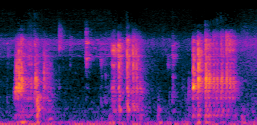
\includegraphics[width=0.7\linewidth]{brux_spec}
    \caption{ spectrogram van tanden knarsen (duratie 3s mono)}
    \label{fig:mil spectrogram of teeth grinding (duration 3s)}
\end{figure}

De verzamelde data kan worden opgesplitst in kleinere fragmenten .
De  fragmenten kan vergroot worden met Time shifting, pitch shifting and het gebruik van Gauss-ruis voor de aanpassing van de inputlaag .




\bigbreak
Wanneer de data aangepast en verzameld is kan ze worden omgezet in spectrogrammen door het gebruik van Time en frequency masking .
Deze methodes zorgen voor een tweeledig voordeel, namelijk, het model is resistenter tegen ontbrekende data omdat het model zich moet focussen op de meest essentiële features . 
Het andere element is de extra uitbreiding van de hoeveelheid spectrogrammen .
Wanneer de spectrogrammen zijn aangemaakt kunnen ze worden gelabeld .
De spectrogrammen geven de mogelijkheid om het als een image-classificatie probleem op te lossen .

\bigbreak
Alle data zal worden opgeslaan met gebruik van MongoDb in de aangepaste vorm om de waarborg van privacy van de subjecten te garanderen .
\bigbreak

Wanneer de data is verwerkt en opgeslaan kan een werkend model worden gebouwd, waar factoren zoals precisie en herinnering belangerijke factoren zijn om het juiste model te selecteren .
Het werkend model zal worden geimplementeerd in een mobiele applicatie als proof of concept .
De grootste hoeveelheid van de beschikbare tijd zal hieraan worden gespendeerd .


\subsection{proof of concept}

Het proof of concept zal gebouwd worden met gebruik van het python framework Kivy .
De applicatie zal de mogelijkheid hebben om geluid op te nemen en de user te vertellen hoeveel SB gebeurtenissen plaatsgevonden hebben .

\bigbreak
Als samenvatting, data zal worden verzameld van SB en niet-SB subjecten met een aantal soorten kauw-gerelateerde geluiden . Die data zal worden verwerkt en omgevormd tot spectrogrammen .
De spectrogrammen laten toe om een image-classificatie probleem te maken .
Het model zal worden geimplementeerd in een mobiele applicatie met Kivy .







\section{Verwachte conclusies}

% TODO: (fase 6) beschrijf wat je verwacht uit je onderzoek en waarom (bv. volgens je literatuuronderzoek is softwarepakket A het meest gebruikte en denk je dat het voor deze casus ook het meest geschikt zal zijn). Natuurlijk kan je niet in de toekomst kijken en mag je geen alternatieve mogelijkheden uitsluiten. In de praktijk gebeurt het ook vaak dat een onderzoek tot verrassende resultaten leidt, dat maakt het proces nog interessanter!

De creatie van een model dat hoogst waarschijnlijk gebaseerd is op een convolutioneel netwerk dat SB gebeurtenissen kan ontdekken en de duur meten door het ontdekken van het knarsen van tanden, dat een symptoom is van SB .

Het model wordt gebruikt in een POC mobiele applicatie dat hoogst waarschijnlijk op basis van Kivy werkt .









%------------------------------------------------------------------------------
% Referentielijst
%------------------------------------------------------------------------------
% TODO: (fase 4) de gerefereerde werken moeten in BibTeX-bestand
% bibliografie.bib voorkomen. Gebruik JabRef om je bibliografie bij te
% houden.

\phantomsection
\printbibliography

\end{document}
